\section*{Questionnaire}

\noindent\textbf{What is the issue that interests you?}
\newline\hspace{10mm}Precision medicine.

\noindent\textbf{Why does it interest you?}
\newline\hspace{10mm}Mostly just from curiosity that stems  from a talk hosted by the International Conference on Functional Programming called Precision Medicine.

\noindent\textbf{What stake (or personal interest) do you have in the issue?}
\newline\hspace{10mm}I don’t necessarily have any financial stakes in the manner, or other personal interests. I once wondered if this could be used to hep my Grandma -who had cancer- but this isn’t relevant anymore.

\noindent\textbf{What do you already know about this issue?}
\newline\hspace{10mm}That precision medicine is -broadly- based on applying computation to problems, searching for answers that may be infeasible for humans to manually compute.

\noindent\textbf{What is your position on this issue?}
\newline\hspace{10mm}My current position is that I’m simply curious about the matter.

\noindent\textbf{What are opponents’ positions?}
\newline\hspace{10mm}From what I understand, that limited government funding would be better spent on other projects. There seems to be a common theme that government or public investments should be focused on prevention.

\noindent\textbf{Is there common ground on the issue? What would it be?}
\newline\hspace{10mm}Not that I’m aware of, so no.

\noindent\textbf{Post an image that best relays your chosen issue in the form of a visual.}\newline
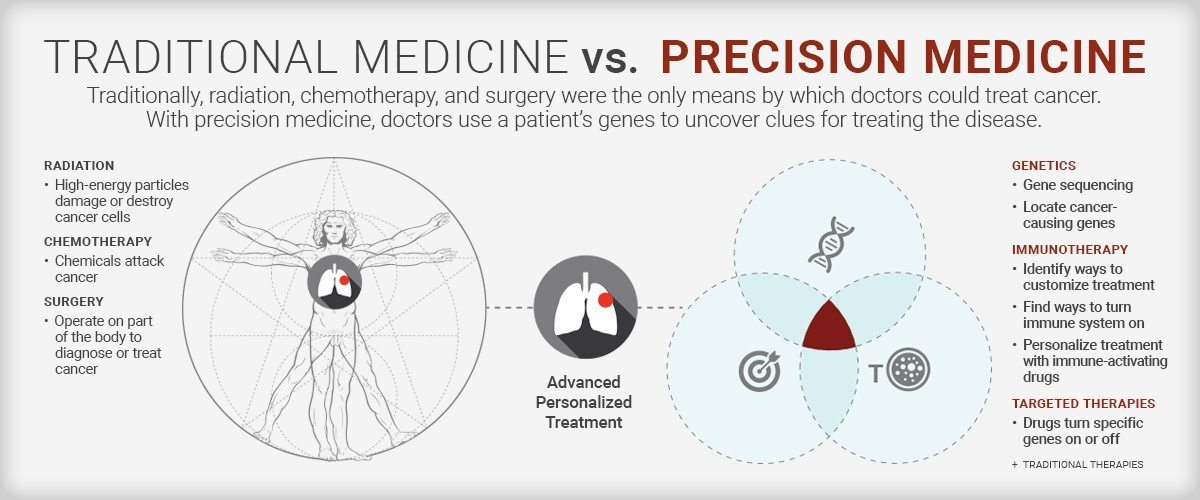
\includegraphics[scale=0.4]{../assets/infographic1.jpg}
\textbf{(Source: \url{https://healthmatters.nyp.org/precision-medicine/}.)}

\section*{Elaboration}

I don’t know if my chosen research topic is very conducive to the assumptions of the above questions. My research topic is about a model used in medicine, it isn’t necessarily an ‘issue’, just as much as evidence based medicine or a mathematical model is an issue.

There is a contrast between precision medicine and our current model of evidence based medicine, where trials must be conducted to test the efficacy of such against the current standard of treatment, which is established VIA generalizations of the applicable demographic.

For instance, consider a disease where the current standard in treatment is so ineffective that your chances of survival is, should I say, grim. Now, imagine the development of a new treatment based on some new fundamental discovery or other innovation that overall, significantly improves your chances of survival. 

With our current system of evidence based medicine, trials must be performed to verify the efficacy against the current standard of treatment, which implies a moral dilemma. If the aforementioned claims are true, half of your patients must undergo the current standard of treatment and therein be effectively condemned to death.\textsuperscript{(For a real life example of this dilemma, see “A Future Of Medicine” by Dr. Bernard.)}

More relevant to my chosen topic. Efficacy is based on generalizations of the applicable demographic, which doesn’t necessarily accommodate differences between yourself and the general population. As Dr. Bernard points out in A Future Of Medicine, if a trial was done on a bunch of men, clinical experience suggests that there will be differences for women taking the same medication.\textsuperscript{(Bernard)}

But what Dr. Bernard is aiming for is a -more ideal- hypothetical replacement to our current standard of evidence based medicine that is founded on computer modeling -technology that, as he points out, will probably not be available in our lifetime.

Where does precision medicine and its issues fit within this spectrum?

Precision medicine may share similarities with Dr. Bernard’s hypothetical system, i.e. that computer modeling may be used to uncover avenues with medical applications. But it isn’t necessarily a replacement, and may also suffer from the same flaws if derived from datasets sourced from the general population. 

Perhaps,  as Jacques S Beckmann wrote,
\begin{quotation}
`This ``one size fits all'' approach [of the current standard] can provide inadequate solutions for outliers. Such outliers, which are far from an oddity as all of us fall into this category for some traits, can be better managed using precision medicine. Here, we argue that it is necessary and possible to bridge between precision medicine and evidence-based medicine.'\textsuperscript{(Beckmann)}
\end{quotation}

Therefore, I consider precision medicine to be a tool to be used alongside our current standard in treatment. A tool that is flawed, just as our current standard in medicine is flawed. 

There are also indirect issues pertaining to precision medicine. Depending on your view of government support.

For instance, in his 2015 state of the union address, President Barack Obama remarked on his initiative in precision medicine. Yet some critics say that limited public funds would be better spent on more traditional solutions, such as in disease prevention, which would benefit a greater portion of the population. As John H Coote wrote,
\begin{quotation}
    ``We believe precision medicine is not the route to a healthy world and instead urge a renewed and increased focus on public health and prevention.''\textsuperscript{(Coote)}
\end{quotation}

In the same speech, President Barack Obama remarked about affordability with regards to precision medicine. Yet critics say that the drug he cited required significant costs in the development of such.\textsuperscript{(Interlandi)}

Personally I think, if precision medicine is a technology that benefits from economies of scale, then costs should therefore decrease over time as such becomes widely implemented while costs factors are optimized. 

There are also technical issues. For instance, documented medical information needs to be conducive to computer processing. Format wise, there are competing solutions such as the Biological Expression Language.\textsuperscript{(Slater)} But still, the issue remains, preexisting literature needs to be translated into such formats, either manually (such as VIA crowdsourcing) or in an automated manner, all of which have their own pros and cons. 

For a perhaps expert option on this matter, lookup ``Matt Might, precision medicine'' in YouTube. He has a Ph.D in computer science, and is a director of a medical department in precision medicine at UAB.\textsuperscript{(Might)} Overall, from what I've seen, he has frequently remarked about the challenges of essentially integrating a legacy system into this new framework of computer processing.


Then there is the issue of actually modeling the problem; which bears overlap with another emerging field called systems biology. But I digress.


\section*{Author's Note}

I hope this adequately conveys the multitude of issues pertaining to precision medicine (PM). My replies to the questionnaire was brief, but I thought it would be better to answer such questions directly, then I delved into the unique issues specific to PM (that I'm currently aware of). The latter part of my essay answers the questions in a less direct manner, hence the two parts to this essay. The latter includes a preliminary introduction to our current standard in medicine, and where PM may fit into this larger framework.

I have a background in IT, including general programming experience. So I was planning on delving into the more technical side of this, but my essay was already getting a bit long at this point, so it got cut short. 




